\documentclass[12pt,letterpaper,titlepage]{article}
\usepackage[latin1]{inputenc}
\usepackage{fullpage}
\usepackage{amsmath}
\usepackage{amsfonts}
\usepackage{amssymb}
\usepackage{tikz}
\usepackage{pgf}
\usetikzlibrary{arrows,automata}
\author{Dimitri Demergis \\ Jason Lee \\ Stephen Lombardi \\ Marcus McCurdy}
\title{CS544 Group 5 Protocol}
\begin{document}

\maketitle

\tableofcontents

\pagebreak

\section{Introduction}
This paper defines a media streaming protocol that allows a properly implemented server to stream media to connected clients. Clients are able the join at any time during the streaming process and may be required to authenticate themselves to the server. The protocol is designed to deal with arbitrary streaming data types, including live or prerecorded video and/or audio.

\section{Messages}
\subsection{Client-to-Server Messages}
\subsubsection{SessionRequestMessage}
	\begin{description}
	\item[Description] \hfill \\
		This message is sent by the client to the server.  It is used to notify the server that it 
		should provision a new streaming session. It also includes the version numbers of the 
		protocol the client supports.
	\item[Message Format] \hfill \\
	\begin{tabular}{ | c | c | }
		\hline
		1 byte & 1 byte \\
		\hline
		Message ID &  Version Number \\
		\hline
	\end{tabular}
	\item[Message Field Definitions] \hfill \\
	\begin{tabular}{ | p{3cm} | p{1.5cm} | p{8cm} | }
		\hline
		Field Name & Data Type & Definition \\
		\hline
		Message ID & byte & Contains the Message ID number. \newline Always set to 1 for this message. \\
		\hline
		Version Number & byte & Identifies the latest version of the protocol supported by the client.
						\newline 1 = Version 1.0 \\
		\hline
	\end{tabular}
	\end{description}
\subsubsection{ChallengeResponseMessage}
	\begin{description}
	\item[Description] \hfill \\
		This message is sent from the client to the server as part of the authentication process.  
		Upon receiving the ChallengeMessage, the client passes the received challenge value 
		(as well as its own password) to a hash function and sends the result back to the server.
	\item[Message Format] \hfill \\
	\begin{tabular}{ | c | c | c | }
		\hline
		1 byte & 1 byte & 4 bytes \\
		\hline
		Message ID & Session ID &  Challenge Response \\
		\hline
	\end{tabular}
	\item[Message Field Definitions] \hfill \\
	\begin{tabular}{ | p{3cm} | p{1.5cm} | p{8cm} | }
		\hline
		Field Name & Data Type & Definition \\
		\hline
		Message ID & byte & Contains the Message ID number. 
					\newline Always set to 4 for this message. \\
		\hline
		Session ID & byte & Contains the Session ID number pertaining to this message. \\
		\hline
		Challenge Response & int & Contains the client's challenge response. \\
		\hline
	\end{tabular}
	\end{description}
\subsubsection{DisconnectMessage}
	\begin{description}
	\item[Description] \hfill \\
		This message is sent from the client to the server to indicate that the connection should be closed.
	\item[Message Format] \hfill \\
	\begin{tabular}{ | c | c | c | }
		\hline
		1 byte & 1 byte \\
		\hline
		Message ID & Session ID \\
		\hline
	\end{tabular}
	\item[Message Field Definitions] \hfill \\
	\begin{tabular}{ | p{3cm} | p{1.5cm} | p{8cm} | }
		\hline
		Field Name & Data Type & Definition \\
		\hline
		Message ID & byte & Contains the Message ID number. 
					\newline Always set to 6 for this message. \\
		\hline
		Session ID & byte & Contains the Session ID number pertaining to this message. \\
		\hline
	\end{tabular}
	\end{description}
\subsubsection{ThrottleMessage}
	\begin{description}
	\item[Description] \hfill \\
		This message is sent from the client to the server to control the rate of data being sent to the client. It can be used to increase or decrease rate of transmission.
	\item[Message Format] \hfill \\
	\begin{tabular}{ | c | c | c | }
		\hline
		1 byte & 1 byte & 4 bytes \\
		\hline
		Message ID & Session ID & Rate \\
		\hline
	\end{tabular}
	\item[Message Field Definitions] \hfill \\
	\begin{tabular}{ | p{3cm} | p{1.5cm} | p{8cm} | }
		\hline
		Field Name & Data Type & Definition \\
		\hline
		Message ID & byte & Contains the Message ID number. 
					\newline Always set to 7 for this message. \\
		\hline
		Session ID & byte & Contains the Session ID number pertaining to this message. \\
		\hline
        Rate & float & Indicates the client's desired rate of transmission in bytes per second. \\
        \hline
	\end{tabular}
	\end{description}

\subsection{Server-to-Client Messages}
\subsubsection{SessionMessage}
	\begin{description}
	\item[Description] \hfill \\
		This is the servers reply to the SessionRequestMessage. It tells the client what version of 
		the protocol that will be used during the streaming session. It also contains the session id 
		that will be used in further communication with the server.
	\item[Message Format] \hfill \\
	\begin{tabular}{ | c | c | c | c | c | }
		\hline
		1 byte & 1 byte & 1 byte & 1 byte & $n$-bytes \\
		\hline
		Message ID & Session ID &  Version Number & Type Length & Stream Type \\
		\hline
	\end{tabular}
	\item[Message Field Definitions] \hfill \\
	\begin{tabular}{ | p{3cm} | p{1.5cm} | p{8cm} | }
		\hline
		Field Name & Data Type & Definition \\
		\hline
		Message ID & byte & Contains the Message ID number. \newline Always set to 2 for this message. \\
		\hline
		Session ID & byte & Contains the Session ID number pertaining to this connection. \\
		\hline
		Version Number & byte & Identifies the protocol version to be used in this connection.
						\newline 1 = Version 1.0 \\
		\hline
        Type Length & byte & Contains the value of $n$, the length of the Stream Type field. \\
        \hline
        Stream Type & variable & An ASCII-encoded string describing the encoding format and data type of the stream. \\
        \hline
	\end{tabular}
	\end{description}
\subsubsection{ChallengeMessage}
	\begin{description}
	\item[Description] \hfill \\
		This message is sent from the server to the client to begin the authentication process.  
		The message contains a challenge value to be generated by the server.  This message marks 
		the transition from the Connecting state to the Authentication state. 	
	\item[Message Format] \hfill \\
	\begin{tabular}{ | c | c | c | }
		\hline
		1 byte & 1 byte & 4 bytes \\
		\hline
		Message ID & Session ID &  Challenge Value \\
		\hline
	\end{tabular}
	\item[Message Field Definitions] \hfill \\
	\begin{tabular}{ | p{3cm} | p{1.5cm} | p{8cm} | }
		\hline
		Field Name & Data Type & Definition \\
		\hline
		Message ID & byte & Contains the Message ID number. 
					\newline Always set to 3 for this message. \\
		\hline
		Session ID & byte & Contains the Session ID number pertaining to this message. \\
		\hline
		Challenge Value & int & Contains a randomly-generated challenge value. \\
		\hline
	\end{tabular}
	\end{description}
\subsubsection{ChallengeResultMessage}
	\begin{description}
	\item[Description] \hfill \\
		This message is sent from the server to the client to complete the authentication process.  
		Upon receiving the ChallengeResponseMessage, the server compares the result received from 
		the client to its own result, and informs the client of success or failure.
	\item[Message Format] \hfill \\
	\begin{tabular}{ | c | c | c | }
		\hline
		1 byte & 1 byte & 1 byte \\
		\hline
		Message ID & Session ID &  Challenge Result \\
		\hline
	\end{tabular}
	\item[Message Field Definitions] \hfill \\
	\begin{tabular}{ | p{3cm} | p{1.5cm} | p{8cm} | }
		\hline
		Field Name & Data Type & Definition \\
		\hline
		Message ID & byte & Contains the Message ID number. 
					\newline Always set to 5 for this message. \\
		\hline
		Session ID & byte & Contains the Session ID number pertaining to this message. \\
		\hline
		Challenge Result & byte & Contains the result of the challenge process.
						\newline 0 = Failure 
						\newline 1 = Success \\
		\hline
	\end{tabular}
	\end{description}
\subsubsection{AuthenticationErrorMessage}
	\begin{description}
	\item[Description] \hfill \\
		This message is sent from the server to the client to notify the client of an error in 
		completing the authentication process. This message contains an error code in order to 
		properly inform the client of the nature of the error. This message transitions the protocol
		state from Authenticating to Disconnected.
	\item[Message Format] \hfill \\
	\begin{tabular}{ | c | c | c | }
		\hline
		1 byte & 1 byte & 4 bytes \\
		\hline
		Message ID & Session ID & Error Code \\
		\hline
	\end{tabular}
	\item[Message Field Definitions] \hfill \\
	\begin{tabular}{ | p{3cm} | p{1.5cm} | p{8cm} | }
		\hline
		Field Name & Data Type & Definition \\
		\hline
		Message ID & byte & Contains the Message ID number. 
					\newline Always set to 9 for this message. \\
		\hline
		Session ID & byte & Contains the Session ID number pertaining to this message. \\
		\hline
		Error Code & int & Contains the code for the error that occurred during the authentication process. \\
		\hline
	\end{tabular}
	\end{description}	
\subsubsection{StreamMessage}
	\begin{description}
	\item[Description] \hfill \\
		These messages are sent while the protocol is in the streaming state. They contain the 
		actual data that is being streamed. The message consists of a message ID identifying it as a data message, a session ID identifying the session, a four-byte data length field, and a variable $n$-byte data chunk.
	\item[Message Format] \hfill \\
	\begin{tabular}{ | c | c | c | c | c | c | }
		\hline
		1 byte & 1 byte & 1 byte & 4 bytes & $n$ bytes & 1 byte \\
		\hline
		Message ID & Session ID & Sequence Number & Data Length & Encoded Data & CRC \\
		\hline
	\end{tabular}
	\item[Message Field Definitions] \hfill \\
	\begin{tabular}{ | p{3cm} | p{1.5cm} | p{8cm} | }
		\hline
		Field Name & Data Type & Definition \\
		\hline
		Message ID & byte & Contains the Message ID number. 
					\newline Always set to 5 for this message. \\
		\hline
		Session ID & byte & Contains the Session ID number pertaining to this message. \\
        \hline
        Sequence Number & byte & Sequence number for this message. \\
		\hline
		Data Length & int & Contains the value of $n$. \\
		\hline
        Encoded Data & variable & Encoded stream data. \\
        \hline
        CRC & byte & Cyclic redundancy check for the packet. \\
        \hline
	\end{tabular}
	\end{description}
	
	\subsubsection{StreamErrorMessage}
	\begin{description}
	\item[Description] \hfill \\
		This message may be sent while the protocol is in the streaming state. It signifies an unrecoverable
		error during the streaming process. It causes the protocol to transition from the streaming to
		disconnected state.
	\item[Message Format] \hfill \\
	\begin{tabular}{ | c | c | }
		\hline
		1 byte & 1 byte  \\
		\hline
		Message ID & Session ID  \\
		\hline
	\end{tabular}
	\item[Message Field Definitions] \hfill \\
	\begin{tabular}{ | p{3cm} | p{1.5cm} | p{8cm} | }
		\hline
		Field Name & Data Type & Definition \\
		\hline
		Message ID & byte & Contains the Message ID number. 
		\newline Always set to 10 for this message. \\
		\hline
		Session ID & byte & Contains the Session ID number pertaining to this message. \\
	        \hline
	\end{tabular}
	\end{description}

\section{DFA}
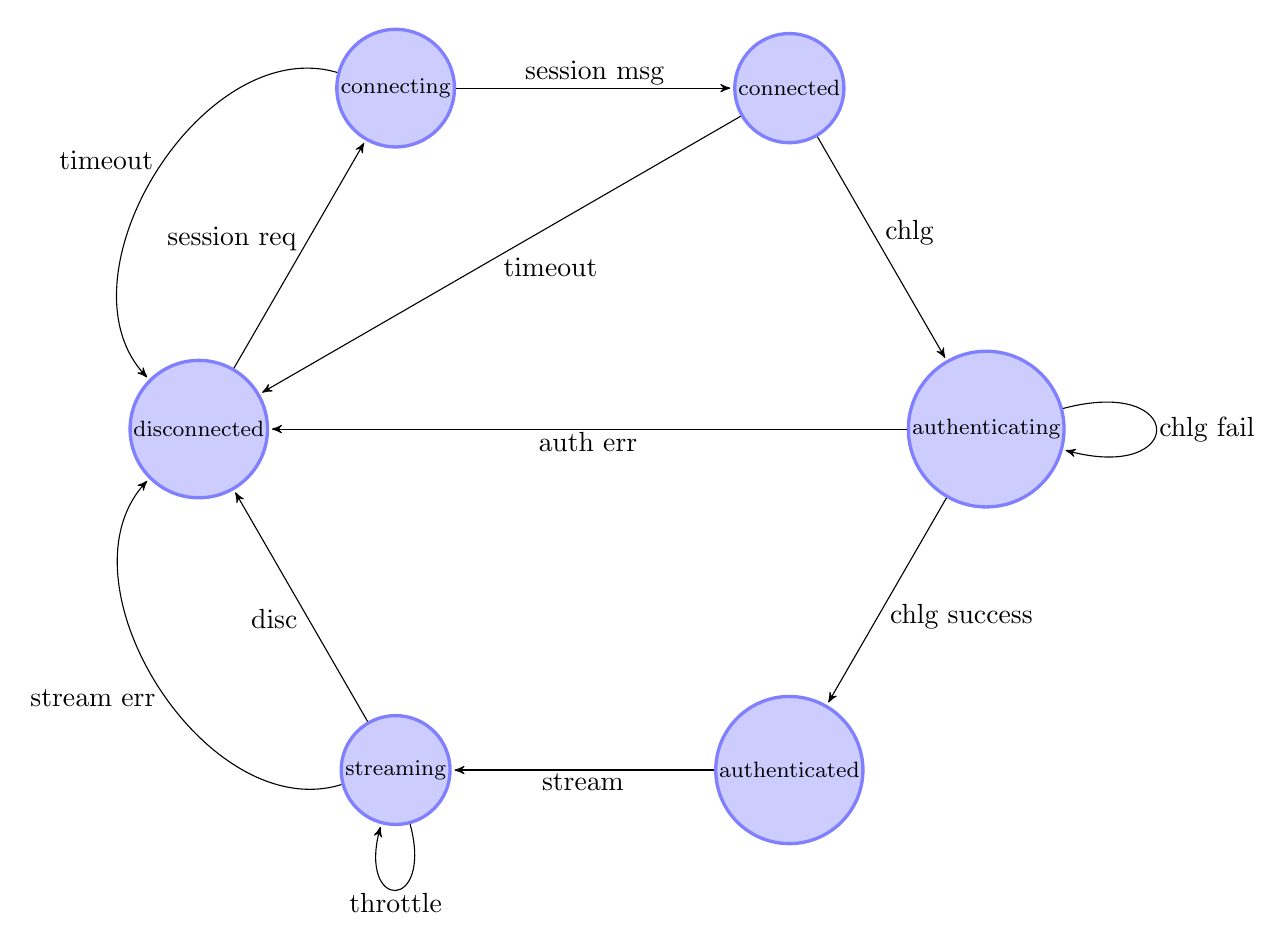
\begin{tikzpicture}[->,>=stealth',shorten >=1pt,auto,bend angle=75,inner sep=1pt, every state/.style={draw=blue!50,very thick,fill=blue!20, font=\footnotesize}]

\foreach \name/\text/\angle in {1/disconnected/180, 2/connecting/120, 3/connected/60, 4/authenticating/0, 5/authenticated/300, 6/streaming/240}
\node[state,xshift=10cm,yshift=2cm](\name) at (\angle:5cm) {\text};

\path 
	(1) edge				node {session req} 	(2)
	(2) edge				node {session msg} 	(3)
	      edge [bend right]		node[swap] {timeout} 		(1)	
	(3) edge				node {chlg}		(4)
	      edge				node {timeout}		(1)	
	(4) edge 				node {chlg success}	(5)
	      edge [loop right]		node {chlg fail}          (4)
	      edge 				node {auth err}          (1)
	(5) edge				node {stream}		(6)
	(6) edge				node {disc}		(1)
	      edge [loop below]	node {throttle}		(6)
	      edge [bend left]		node {stream err}	(1)	      	
	
	;

\end{tikzpicture}

%session request id = 1
% ChallengeResponseMessage = 4
% Disconnect = 6
% Throttle = 7
%SessionMessage = 2
%ChallengeMessage = 3
% ChallengeResult = 5
%auth err = 9
%stream = 5

\section{Extensibility}
Protocol version information is included in connection messages so that the protocol version used by both sides can be established during the configuration phase.  This allows future improvements to the protocol to be implemented without rendering existing client applications unusable. In addition to this, the type of media and encoding that the stream uses are sent to the client as an ASCII-encoded string. This allows clients and servers to implement additional encodings as they are developed without updates to the protocol.

\section{Security}
This protocol uses a CHAP-like handshaking protocol for authentication of clients.  After the connection has been established, the server sends a challenge message to the client.  Both the client and server pass a password through a pre-determined hash function, and the server checks the results and informs the client of success or failure.

\section{Reliability}
Due to the real-time nature of the protocol, it does not attempt to retransmit any lost packets. It does, however, provide sequence number on all data messages in order to ignore any packets which have reached the client after a more recently sent packet. In addition to this, each data message contains a CRC for basic error checking. When an error is detected, the packet is simply dropped.

\section{Quality of Service}
Streaming media transmission requires careful monitoring of traffic to maintain acceptable levels of loss and to avoid network congestion. These goals are achieved through the ThrottleMessage. The client sends a ThrottleMessage to inform the server that it would like to change the server's rate of transmission to that client. If the network is under a heavy load, the client will observe that packets have been lost in transit by examining sequence numbers. When this occurs, the client will request that the server decrease its current transmission rate to avoid packet loss for other services across the network. This is necessary because UDP will not perform this operation on its own like TCP would. If the client wishes to increase the rate of transmission it may do this as well, but the server is free to ignore any request that is too high.


\end{document}
